%%%%%%%%%%%%%%%%%%%%%%%%%%%%%%%%%%%%%%%%%%%%%%
%                insertmeeting
% 1) Title (something creative & funny?)
% 2) Date (MM/DD/YYYY)
% 3) Location (ex. Hagerty High School)
% 4) People/Committees Present 
% 5) Picture 
% 6) Start Time & Stop Time (ex. 12:30AM to 4:30PM)
%%%%%%%%%%%%%%%%%%%%%%%%%%%%%%%%%%%%%%%%%%%%%%
\insertmeeting 
	{Both Eyes Open} 
	{03/29/22} 
	{Hagerty High School}
	{James, Jensen, Nathan, Ritam}
	{Images/RobotPics/robot.jpg}
	{2:30 - 4:30}
	
\hhscommittee{Software}
\noindent\hfil\rule{\textwidth}{.4pt}\hfil
\subsubsection*{Goals}
\begin{itemize}
    \item Build out a vision program that can calculate the world coordinates of an object. 

\end{itemize} 

\noindent\hfil\rule{\textwidth}{.4pt}\hfil

\subsubsection*{Accomplishments}
One thing that we wanted this year was to automatically pick up blocks during the autonomous period. To accomplish this goal, we would need to detect them using computer vision programs. Since we had lots of experience with OpenCV, we decided to use it again. To begin, we used an EOCV Simulator from DeltaCV for development purposes. Our first goal was to use thresholding and image transformations to get a good detection of the blocks. We did this by using a YCrCb threshold, followed by a erosion and subseuent dilation to create a binary matrix of the detected blocks. Using this matrix as input to findContours(), we were able to create a bounding rectangle around the yellow blocks, regardless of the orientation. The next part proved more difficult. There are numerous ways to calculate the world coordinates of an object from a 2D image. One of the most complex but also most powerful is using homography. However, homography's complex approach and specific conditions meant that we may not be able to successfuly implement it in the time frame. However, we found one approach that would be able to find the X and Y coordinates of an object given the z distance (The distance from the camera to the object). We were able to find the z distance using similar triangles. We measured the pixel width of a block situated at a known distance, 12 in, then used that value to estimate the distance of other blocks based on their pixel width. From that we use RealX = PixelX * (z distance) divided by focal length. Luckily for us, the people at FIRST already calibrated the Logitech C270 for use on FTC systems, providng us the focal length and distortion coefficients. Plugging these values into the code worked well, bringing us to within 3 degrees of error in the calculated heading. 


\begin{figure}[htp]
\centering
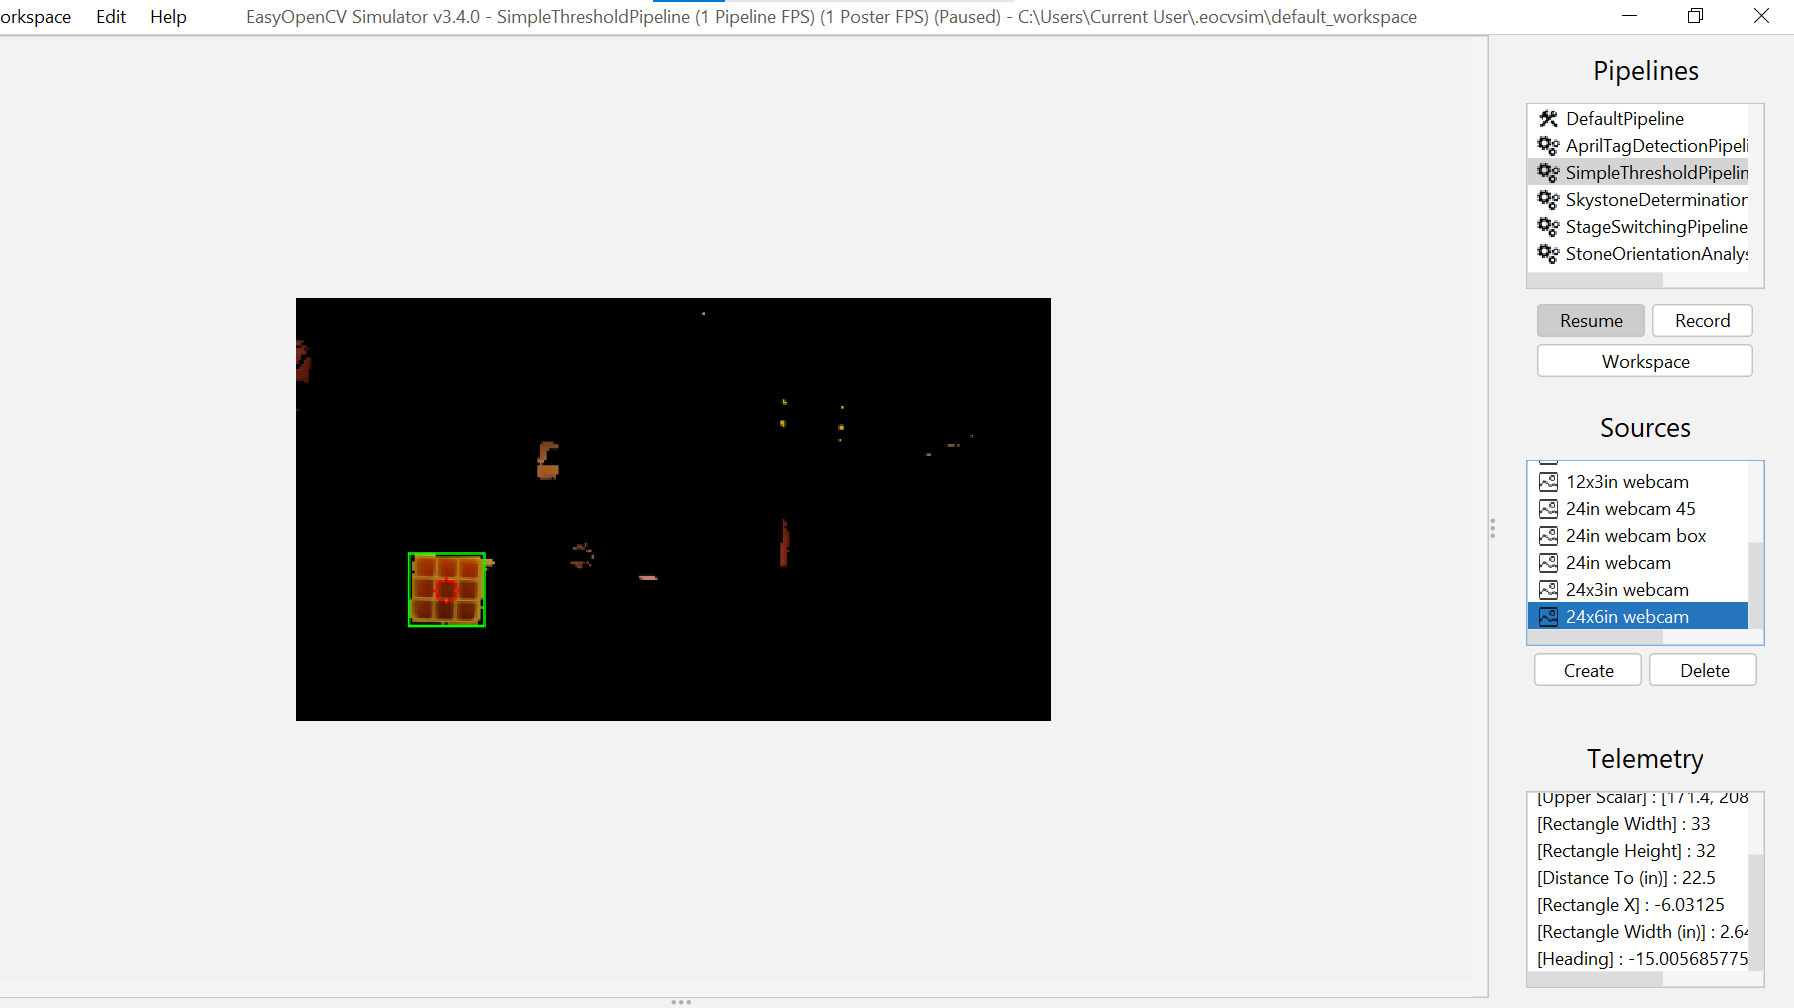
\includegraphics[width=0.95\textwidth, angle=0]{Meetings/March/03-29-22/03-29-22 1.png}
\caption{Our pipeline successfully detected the block at 24 in x 6 in (World coordinates) and correctly calculated the heading to around 15 degrees.}
\label{fig:032922_1}
\end{figure}

\begin{figure}[htp]
\centering
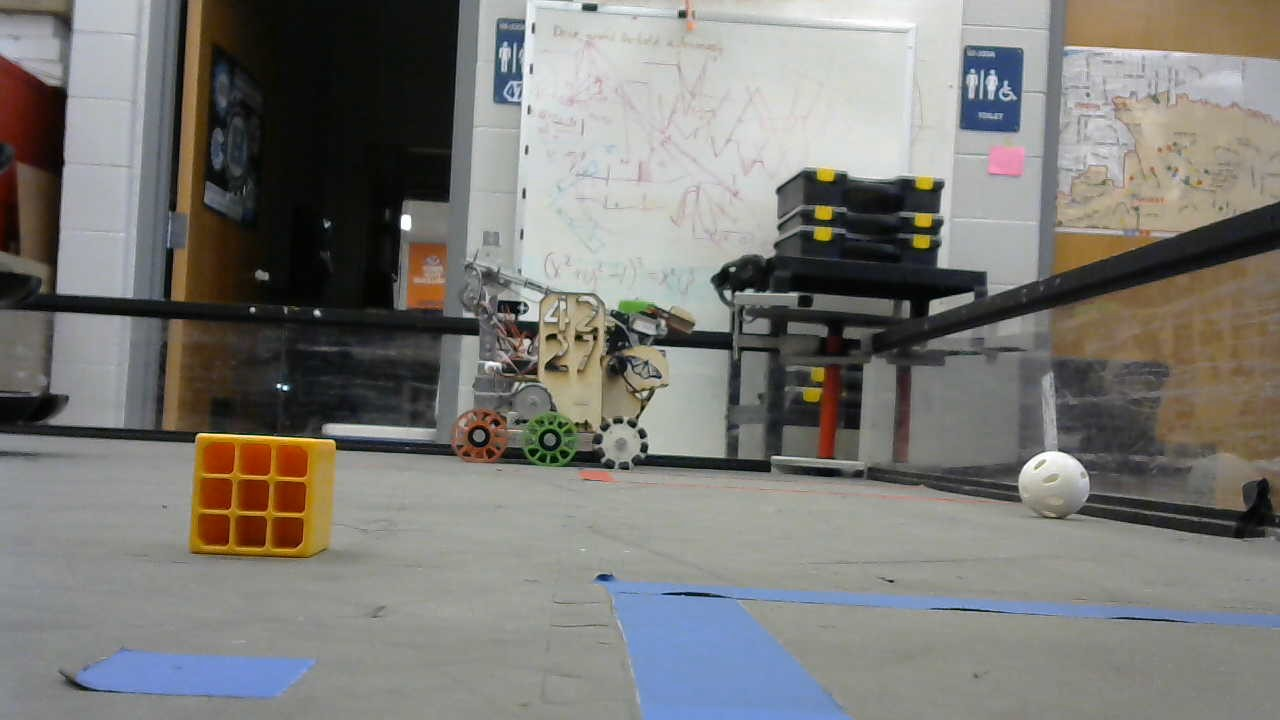
\includegraphics[width=0.95\textwidth, angle=0]{Meetings/March/03-29-22/03-29-22 2.jpg}
\caption{The original image in the picture above before applying OpenCV}
\label{fig:032922_2}
\end{figure}

\begin{figure}[htp]
\centering
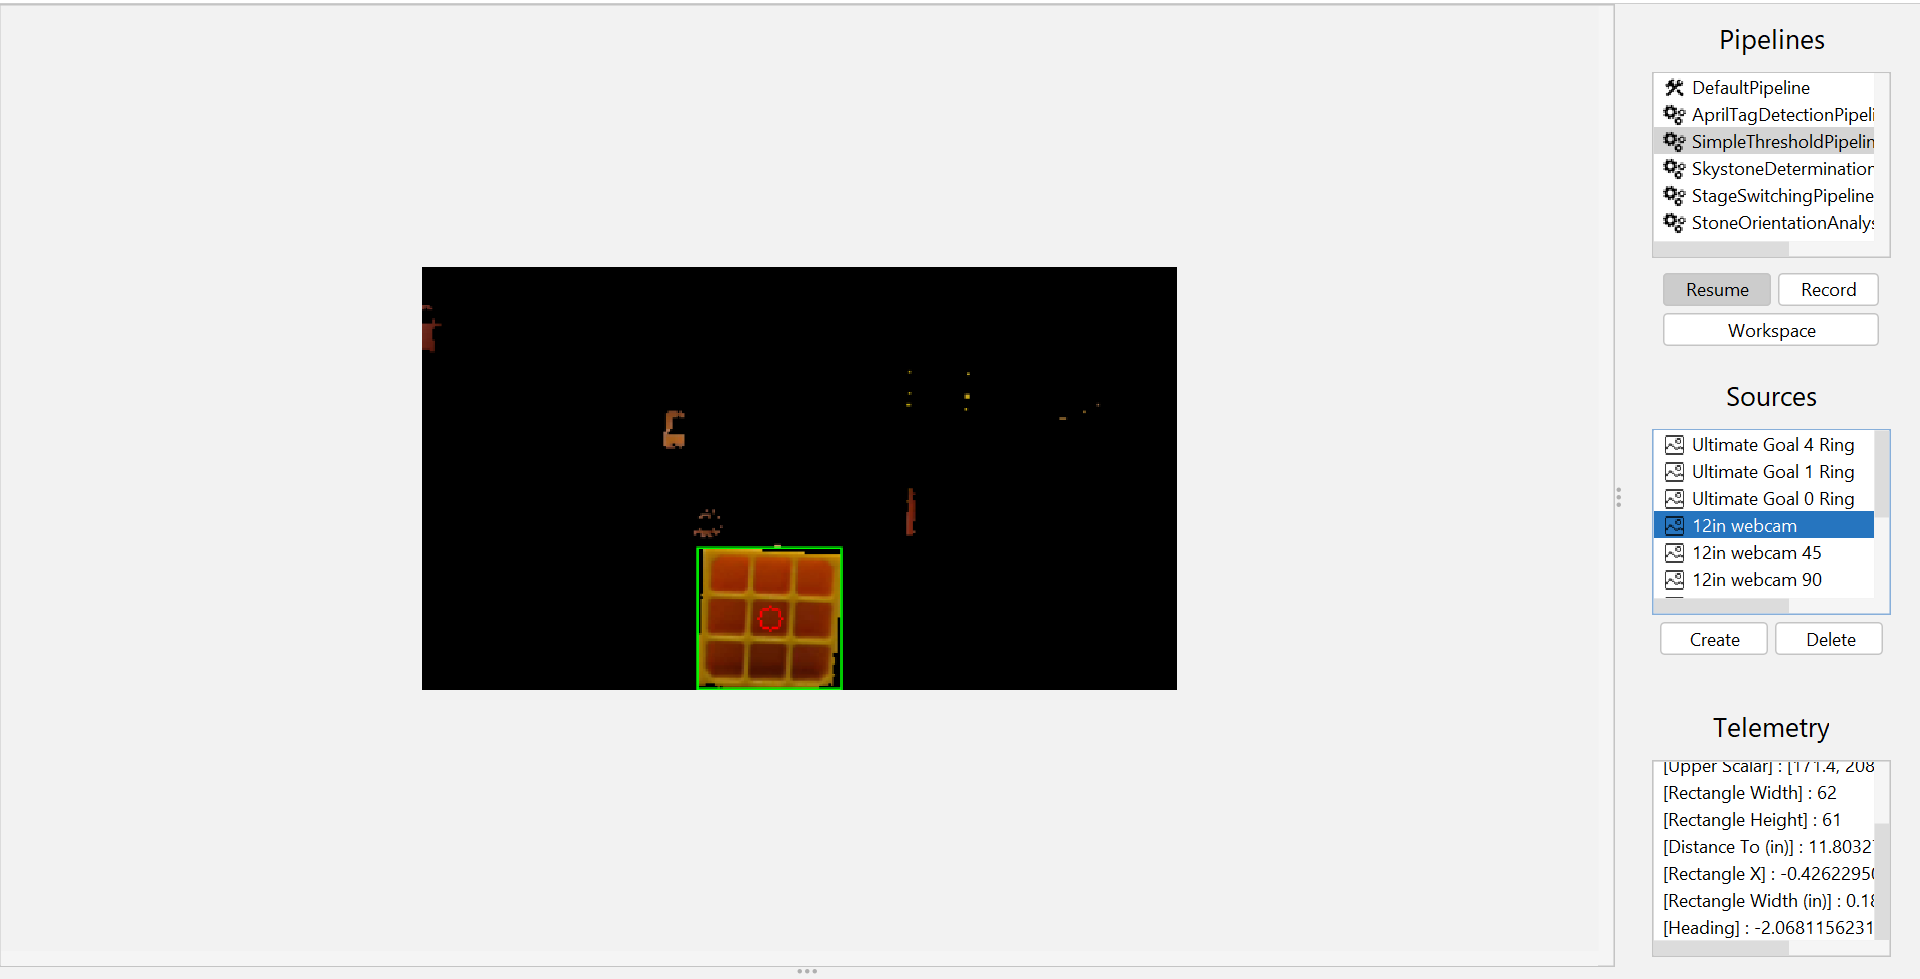
\includegraphics[width=0.95\textwidth, angle=0]{Meetings/March/03-29-22/03-29-22 3.png}
\caption{A block at 12in by 0in that we used to calibrate the known height and pixel width.}
\label{fig:032922_3}
\end{figure}

\begin{figure}[htp]
\centering
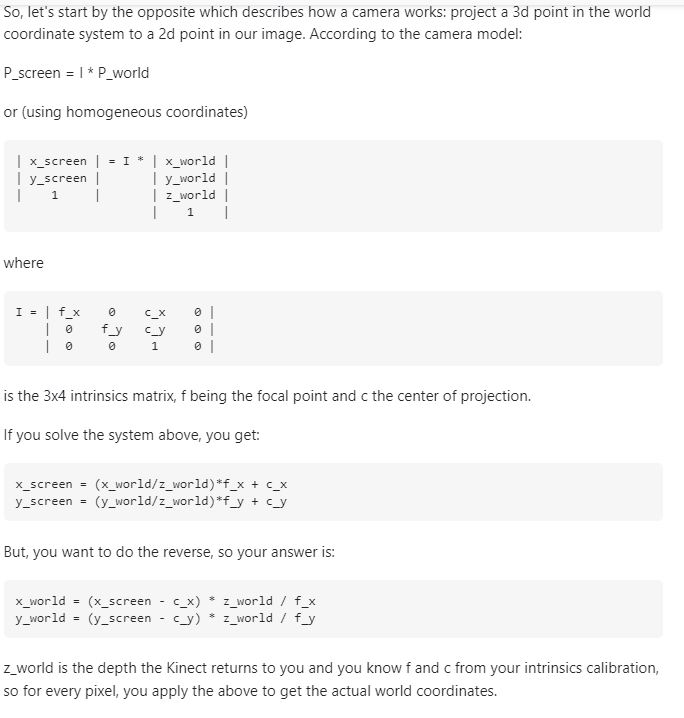
\includegraphics[width=0.95\textwidth, angle=0]{Meetings/March/03-29-22/03-29-22 4.JPG}
\caption{Screnshot from StackOverflow where we got the solution.}
\label{fig:032922_4}
\end{figure}

\begin{figure}[htp]
\centering
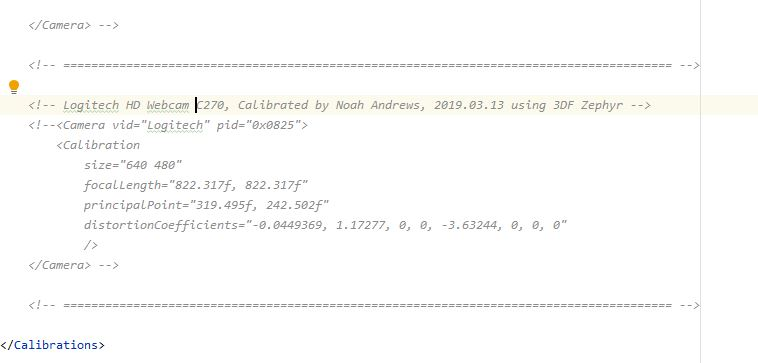
\includegraphics[width=0.95\textwidth, angle=0]{Meetings/March/03-29-22/03-29-22 5.JPG}
\caption{The calibrated camera constants. Thanks Noah Andrews!}
\label{fig:032922_5}
\end{figure}


\whatsnext{
\begin{itemize}
    \item Program navigation methods for the robot to move towards the detected block and calculated heading.
\end{itemize} 
}

